\chapter{कार्बधात्विक रसायन: आबंधन और लिगैंड}\label{ch:b3:organometallic-bonding}

1951 में दो शोध समूहों ने, स्वतंत्र रूप से, सूत्र $\ce{FeC10H10}$ का एक नारंगी, वायु में स्थायी
चूर्ण प्राप्त किया जिसका कोई अर्थ नहीं बनता था: आयरन सामान्यतः कार्बन से स्थायी आबंध नहीं
बनाता, और दो साइक्लोपेन्टाडाइनिल वलयों से एक साथ तो कदापि नहीं। एक वर्ष के भीतर
इसकी संरचना स्थापित हो गई: आयरन दो समांतर वलयों के बीच बैठता है, सभी दस कार्बन
परमाणुओं से समान रूप से आबंधित, एक सैंडविच। फ़ेरोसीन ने
आधुनिक कार्बधात्विक रसायन का द्वार खोला, जिसके उत्प्रेरक आज विश्व के अधिकांश
बहुलक, औषधें और सूक्ष्म रसायन बनाते हैं (\cref{ch:b3:homogeneous-catalysis})।
यह अध्याय समझाता है कि धातुएँ कार्बन मोनोऑक्साइड, फ़ॉस्फ़ीनों, ऐल्कीनों,
वलयों, \omterm{def:b3:organometallic-bonding:carbene}{कार्बीनों} और एक-दूसरे से कैसे आबंधित होती हैं, और \omterm{def:b3:organometallic-bonding:isolobal}{समपालि सादृश्य}
कार्बधात्विक अणुखंडों को कार्बन के कार्बनिक रसायन से कैसे जोड़ता है।

\begin{recall}
प्रथम वर्ष के खंड ने कार्बधात्विक यौगिकों को परिभाषित किया और ग्रीन्यार अभिकर्मकों का उपयोग किया।
द्वितीय वर्ष के खंड ने 18-इलेक्ट्रॉन नियम और संयोजकता इलेक्ट्रॉन गणनाएँ,
हैप्टिसिटी, पश्च-दान सहित $\pi$-ग्राही और $\pi$-दाता लिगैंड, कार्बधात्विक
अभिक्रियाओं के मूल चरण (ऑक्सीकारी योग, अपचायी विलोपन,
निवेशन) और अणुखंड कक्षक प्रस्तुत किए। \Cref{ch:b3:group-theory-applied} ने
कार्बोनिलों के \omterm{def:b3:group-theory-applied:activity}{अवरक्त-सक्रिय} CO तनन गिने और सममिति-अनुकूलित
संयोजन बनाए; \cref{ch:b3:complex-spectra-magnetism} ने चुंबकीय आघूर्णों को
अयुग्मित इलेक्ट्रॉनों से संबंधित किया।
\end{recall}

\begin{omfigure}
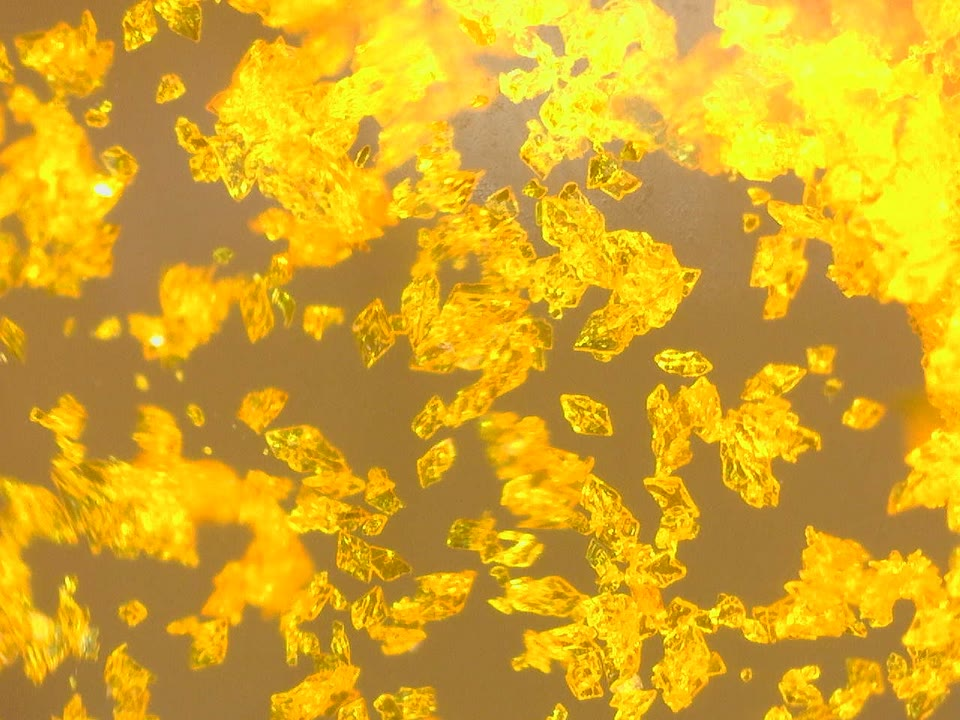
\includegraphics[width=0.5\linewidth]{images/book4/ferrocene-crystals.jpg}

{\small फ़ेरोसीन, $\ce{Fe(C5H5)2}$, के क्रिस्टल: एक नारंगी कार्बधात्विक यौगिक,
वायु में स्थायी, जो हल्का गर्म करने पर ऊर्ध्वपातित हो जाता है।}
\end{omfigure}

\section{इलेक्ट्रॉन गणना और ऑक्सीकरण अवस्थाएँ}

\begin{method}[इलेक्ट्रॉन गणना, दो ढंगों से]\label{met:b3:organometallic-bonding:count}
\begin{enumerate}
  \item उदासीन-लिगैंड (सहसंयोजी) विधि: धातु अपनी समूह संख्या जितने
        इलेक्ट्रॉन लाती है; प्रत्येक लिगैंड, उदासीन मानकर, 1 (H, \ce{CH3}, Cl,
        $\eta^1$-ऐलिल) या 2 (CO, \ce{PR3}, ऐल्कीन) या अधिक ($\eta^5$-\ce{C5H5} 5, $\eta^6$-\ce{C6H6} 6) लाता है; प्रति
        धातु--धातु आबंध एक जोड़िए और समग्र आवेश के लिए संशोधन कीजिए।
  \item आयनिक विधि: H, \ce{CH3}, Cl, \ce{C5H5} जैसे लिगैंड ऋणायनों के रूप में गिने जाते हैं (2, 2,
        2 और 6 इलेक्ट्रॉन), और धातु परिणामी $d^n$ धनायन के रूप में; उदासीन लिगैंड
        पहले की तरह।
  \item दोनों समान योग देती हैं; आयनिक विधि ऑक्सीकरण अवस्था
        और $d^n$ गणना भी देती है।
\end{enumerate}
\end{method}

\begin{example}[गणना]\label{ex:b3:organometallic-bonding:count}
$\ce{Fe(CO)5}$: $8 + 5 \times 2 = 18$, आयरन(0), $d^8$। फ़ेरोसीन: उदासीन विधि $8 + 2 \times 5 = 18$; आयनिक विधि
$\ce{Fe^{2+}}$ ($d^6$, 6) $+ 2 \times 6$ ($\ce{C5H5-}$) $= 18$, आयरन(II)। $\ce{Mn2(CO)10}$: प्रत्येक Mn $7 + 5 \times 2 + 1$ (Mn--Mn
आबंध) $= 18$। वर्ग-समतलीय $d^8$ संकुलों, जैसे $\ce{[PtCl4]^{2-}}$ या विल्किन्सन उत्प्रेरक
$\ce{RhCl(PPh3)3}$, में 16 इलेक्ट्रॉन होते हैं: उनका रिक्त $p_z$-सदृश कक्षक भरने के लिए बहुत ऊँचा है, और
16-इलेक्ट्रॉन वर्ग-समतलीय संकुल 18-इलेक्ट्रॉन संकुलों जितने ही स्थायी होते हैं।
\end{example}

\section{कार्बोनिल और फ़ॉस्फ़ीन}

\begin{definition}[धातु कार्बोनिल]\label{def:b3:organometallic-bonding:carbonyl}
\emph{धातु कार्बोनिल}\index{धातु कार्बोनिल} कार्बन मोनोऑक्साइड
लिगैंडों वाला संकुल है। \emph{अंतस्थ कार्बोनिल}\index{अंतस्थ कार्बोनिल} कार्बन के माध्यम से
एक धातु से आबंधित होता है; \emph{सेतु कार्बोनिल}\index{सेतु कार्बोनिल}
दो (या तीन) धातुओं को जोड़ता है।
\end{definition}

लुडविग मॉन्ड ने 1890 में पाया कि निकेल सामान्य ताप पर कार्बन मोनोऑक्साइड से
अभिक्रिया करके वाष्पशील द्रव $\ce{Ni(CO)4}$ देता है, जो गर्म करने पर पुनः शुद्ध
निकेल में विघटित हो जाता है: एक परिष्करण प्रक्रम का आधार। कार्बन मोनोऑक्साइड
संक्रमण धातुओं से अपने उच्चतम अधिकृत कक्षक, एक $\sigma$ एकाकी युग्म जो अधिकतर
कार्बन पर है, के माध्यम से बँधता है, और अपने रिक्त $\pi^*$ कक्षकों में, जो कार्बन पर भी
बड़े हैं, इलेक्ट्रॉन ग्रहण करता है।

\begin{definition}[सहक्रियात्मक आबंधन]\label{def:b3:organometallic-bonding:synergic}
\emph{सहक्रियात्मक आबंधन}\index{सहक्रियात्मक आबंधन} लिगैंड से धातु की ओर
$\sigma$ दान और धातु से लिगैंड की ओर $\pi$ पश्च-दान का पारस्परिक सुदृढ़ीकरण है:
दान धातु को इलेक्ट्रॉनों में अधिक समृद्ध और उन्हें लौटाने के लिए अधिक तत्पर बनाता है,
पश्च-दान दान से बने आवेश को हल्का करता है।
\end{definition}

\begin{omfigure}
\begin{tikzpicture}[font=\small, >=Stealth]
  % sigma donation
  \fill[black!70] (0,0) circle (0.14); \node[anchor=north] at (0,-0.4) {M};
  \pic at (0,0) {omlobe={-0.7}{180}};
  \pic at (0,0) {omlobe={0.9}{0}};
  \node[circle, fill=black!40, inner sep=1.6pt] at (1.9,0) {};
  \node[circle, fill=omThm!70, inner sep=1.6pt] at (3.0,0) {};
  \pic at (1.9,0) {omlobe={0.85}{180}};
  \node[font=\scriptsize, anchor=north] at (1.9,-0.25) {C};
  \node[font=\scriptsize, anchor=north] at (3.0,-0.25) {O};
  \draw[->, thick, omThm] (1.4,0.55) to[bend right=30] (0.6,0.55);
  \node[anchor=north] at (1.5,-1.55) {$\sigma$ दान};
  % pi back-donation
  \begin{scope}[xshift=6.0cm]
    \fill[black!70] (0,0) circle (0.14); \node[anchor=north] at (0,-1.1) {M};
    \pic at (0,0) {omdxz};
    \node[circle, fill=black!40, inner sep=1.6pt] at (1.9,0) {};
    \node[circle, fill=omThm!70, inner sep=1.6pt] at (3.0,0) {};
    \pic at (1.9,0) {omp={0.9}{90}};
    \pic at (3.0,0) {omp={-0.6}{90}};
    \draw[->, thick, omThm] (0.6,1.05) to[bend left=30] (1.6,1.05);
    \node[anchor=north] at (1.5,-1.55) {$\pi$ पश्च-दान};
  \end{scope}
\end{tikzpicture}

{\small कार्बन मोनोऑक्साइड का \omterm{def:b3:organometallic-bonding:synergic}{सहक्रियात्मक आबंधन}। बाएँ: कार्बन का एकाकी युग्म ($\sigma$
कक्षक) एक रिक्त $\sigma$-प्रकार धातु कक्षक में दान करता है। दाएँ: एक भरा धातु $d$
कक्षक ($d_{xz}$, अपने दो अक्षों सहित) CO के रिक्त $\pi^*$ कक्षक से अतिव्यापन करता है, जो
कार्बन पर बड़ा है और जिसकी पालियाँ उसकी कलाओं से मेल खाती हैं: इलेक्ट्रॉन वापस एक ऐसे कक्षक में बहते हैं जो
C और O के बीच प्रतिआबंधी है।}
\end{omfigure}

\begin{proposition}[CO तनन आवृत्तियाँ]\label{prop:b3:organometallic-bonding:co-frequency}
कोई धातु CO लिगैंड के $\pi^*$ कक्षकों में जितना अधिक पश्च-दान करती है,
C--O तनन तरंग-संख्या उतनी ही कम होती है।
\end{proposition}

\begin{proof}[तर्क]
CO के $\pi^*$ कक्षक C और O के बीच प्रतिआबंधी हैं: उन्हें भरने से
C--O आबंध दुर्बल होता है, उसका \omterm{def:b3:quantum-model-systems:oscillator}{बल स्थिरांक} घटता है, और फलतः तनन तरंग-संख्या भी, जो
\omterm{def:b3:quantum-model-systems:oscillator}{बल स्थिरांक} के वर्गमूल के अनुसार बदलती है (\cref{ch:b3:rovibrational-spectroscopy})।
$\sigma$ दान ऐसे कक्षक से इलेक्ट्रॉन हटाता है जो C--O के लिए लगभग अनाबंधी (थोड़ा
प्रतिआबंधी) है, जो अपने-आप तरंग-संख्या को थोड़ा बढ़ाता: प्रेक्षित
कमी दिखाती है कि पश्च-दान प्रभावी है।
\end{proof}

मुक्त कार्बन मोनोऑक्साइड का \omterm{def:b3:rovibrational-spectroscopy:anharmonic}{मूल संक्रमण} $\omega_e - 2\omega_ex_e = \qty{2143}{cm^{-1}}$ पर है; उदासीन संकुलों के \omterm{def:b3:organometallic-bonding:carbonyl}{अंतस्थ
कार्बोनिल} मोटे तौर पर 1900 और \qty{2100}{cm^{-1}} के बीच अवशोषित करते हैं,
\omterm{def:b3:organometallic-bonding:carbonyl}{सेतु कार्बोनिल} और भी नीचे। किसी समइलेक्ट्रॉनी श्रेणी के अनुदिश, एक ऋणायनी
कार्बोनिल उदासीन की तुलना में कम तरंग-संख्या पर अवशोषित करता है, धनायनी
अधिक पर: धातु जितनी अधिक इलेक्ट्रॉन-समृद्ध, उतना अधिक पश्च-दान। सममिति (\cref{ch:b3:group-theory-applied}) से
बैंडों की संख्या ज्यामिति देती है।
% ledger: diat:CO.we, diat:CO.wexe

\begin{proposition}[$\pi$ अन्योन्यक्रियाएँ और लिगैंड-क्षेत्र विपाटन]\label{prop:b3:organometallic-bonding:pi-delta}
अष्टफलकीय संकुल में $\pi$-ग्राही लिगैंड $\Delta_{\mathrm o}$ बढ़ाते हैं और $\pi$-दाता लिगैंड
उसे घटाते हैं।
\end{proposition}

\begin{proof}
$e_g$ कक्षकों में केवल $\sigma$ सममिति है। $t_{2g}$ कक्षक ($d_{xy}$, $d_{xz}$, $d_{yz}$) एक $t_{2g}$ संयोजन से मेल खाते हैं,
जो लिगैंड $\pi$ कक्षकों से बना है: $d_{xy}$ के लिए, $xy$ तल के चारों लिगैंड प्रत्येक
उस तल में अपने M--L अक्ष के लंबवत एक $\pi$ कक्षक प्रस्तुत करते हैं, और
एकांतर चिह्नों वाला संयोजन $d_{xy}$ की सममिति रखता है (शेष
संयोजन $t_{1g}$, $t_{1u}$ और $t_{2u}$ के रूप में रूपांतरित होते हैं और उन्हें कोई $d$ साथी नहीं मिलता)। एक ही
सममिति के दो कक्षक मिश्रित होकर प्रतिकर्षित होते हैं: निचला नीचे धकेला जाता है, ऊपरी ऊपर। एक
$\pi$ ग्राही $t_{2g}$ समुच्चय के ऊपर रिक्त कक्षक प्रस्तुत करता है, जिससे वह नीचे धकेला जाता है: $\Delta_{\mathrm o}$
बढ़ता है। एक $\pi$ दाता उसके नीचे भरे कक्षक प्रस्तुत करता है, जो उसे ऊपर धकेलते हैं: $\Delta_{\mathrm o}$
घटता है। दोनों स्थितियों में $e_g$ स्तर अप्रभावित रहता है।
\end{proof}

इसीलिए CO और \ce{CN-} स्पेक्ट्रमरासायनिक श्रेणी के प्रबल छोर पर हैं, और
हैलाइड तथा हाइड्रॉक्साइड दुर्बल छोर पर, जैसा द्वितीय वर्ष के खंड ने बताया था।

\begin{definition}[टोलमैन प्राचल]\label{def:b3:organometallic-bonding:tolman}
किसी फ़ॉस्फ़ीन का \emph{टोलमैन शंकु कोण}\index{टोलमैन शंकु कोण} उस शंकु का शीर्ष
कोण है, जो एक मानक दूरी पर धातु पर केंद्रित है और जो उसके प्रतिस्थापियों के वान्डरवाल्स पृष्ठों को
ठीक घेर लेता है: उसके आकार का एक माप।
\emph{टोलमैन इलेक्ट्रॉनिक प्राचल}\index{टोलमैन इलेक्ट्रॉनिक प्राचल}
$\ce{Ni(CO)3L}$ के सममित CO तनन की तरंग-संख्या है: फ़ॉस्फ़ीन L जितना अधिक प्रबलता से
दान करता है, यह उतनी ही कम होती है।
\end{definition}

\emergencystretch=3em फ़ॉस्फ़ीनों को उनके प्रतिस्थापियों द्वारा आकार और इलेक्ट्रॉन दान में स्वतंत्र रूप से
समायोजित किया जाता है: ट्राइऐल्किलफ़ॉस्फ़ीन ट्राइऐरिलफ़ॉस्फ़ीनों से प्रबलतर दाता हैं,
फ़ॉस्फ़ाइट सबसे दुर्बल; $\ce{P(tBu)3}$, $\ce{PMe3}$ से कहीं अधिक भारी है। भारी फ़ॉस्फ़ीन
निम्न उपसहसंयोजन संख्याओं और तीव्र लिगैंड वियोजन का पक्ष लेते हैं, इसीलिए वे
इतने अधिक उत्प्रेरकों में दिखते हैं।

\section{$\pi$ लिगैंड}

\begin{definition}[ड्यूआर--चैट--डंकनसन मॉडल]\label{def:b3:organometallic-bonding:dcd}
किसी धातु से ऐल्कीन के आबंधन का \emph{ड्यूआर--चैट--डंकनसन मॉडल}\index{ड्यूआर--चैट--डंकनसन मॉडल}
दो योगदानों को जोड़ता है: $\sigma$ दान, C=C $\pi$ कक्षक से
एक रिक्त धातु कक्षक में, और पश्च-दान, एक भरे धातु $d$ कक्षक से
C=C $\pi^*$ कक्षक में। प्रबल पश्च-दान की इसकी सीमा एक
\emph{धातुसाइक्लोप्रोपेन}\index{धातुसाइक्लोप्रोपेन} है, एक त्रिसदस्यीय वलय
जिसमें दो M--C $\sigma$ आबंध और एक C--C एकल आबंध होते हैं।
\end{definition}

\begin{proposition}[ऐल्कीन में पश्च-दान के परिणाम]\label{prop:b3:organometallic-bonding:dcd}
उपसहसंयोजन C=C आबंध को लंबा करता है और प्रतिस्थापियों को धातु से दूर, पीछे की ओर मोड़
देता है, और पश्च-दान बढ़ने पर यह प्रभाव और अधिक होता है।
\end{proposition}

\begin{proof}[तर्क]
$\pi$ (आबंधी) कक्षक से इलेक्ट्रॉन हटाना और उन्हें $\pi^*$
(प्रतिआबंधी) कक्षक में जोड़ना, दोनों C--C आबंध कोटि घटाते हैं। $\pi^*$ लक्षण का मिश्रण
कार्बनों को $sp^3$ की ओर पुनःसंकरित करता है, जिनके प्रतिस्थापियों से आबंध
धातु से दूर इंगित करते हैं, \omterm{def:b3:organometallic-bonding:dcd}{धातुसाइक्लोप्रोपेन} ज्यामिति की ओर।
\end{proof}

\begin{omfigure}
\begin{tikzpicture}[font=\small, >=Stealth]
  \fill[black!70] (0,0) circle (0.14); \node[anchor=north] at (0,-1.1) {M};
  \pic at (0,0) {omlobe={0.9}{0}};
  \foreach \y in {0.45,-0.45}{\node[circle, fill=black!40, inner sep=1.6pt] at (1.9,\y) {};}
  \pic at (1.9,0.45) {omp={-0.75}{0}};
  \pic at (1.9,-0.45) {omp={-0.75}{0}};
  \draw[->, thick, omThm] (1.3,1.0) to[bend right=30] (0.5,0.6);
  \node[anchor=north] at (1.2,-1.4) {$\sigma$: $\pi$(C=C) $\to$ M};
  \begin{scope}[xshift=5.6cm]
    \fill[black!70] (0,0) circle (0.14); \node[anchor=north] at (0,-1.1) {M};
    \pic at (0,0) {omdxy};
    \foreach \y in {0.45,-0.45}{\node[circle, fill=black!40, inner sep=1.6pt] at (1.9,\y) {};}
    \pic at (1.9,0.45) {omp={-0.75}{0}};
    \pic at (1.9,-0.45) {omp={0.75}{0}};
    \draw[->, thick, omThm] (0.7,0.9) to[bend left=30] (1.5,0.9);
    \node[anchor=north] at (1.2,-1.4) {$\pi$: M $\to$ $\pi^*$(C=C)};
  \end{scope}
\end{tikzpicture}

{\small पार्श्व से बँधे ऐल्कीन का \omterm{def:b3:organometallic-bonding:dcd}{ड्यूआर--चैट--डंकनसन मॉडल} (C=C
ऊर्ध्वाधर, धातु बाईं ओर)। बाएँ: भरा $\pi$ कक्षक (समान कला में दो $p$ कक्षक)
एक रिक्त धातु कक्षक में दान करता है। दाएँ: मेल खाती कलाओं वाला एक भरा धातु $d$ कक्षक
रिक्त $\pi^*$ कक्षक (विपरीत कला में दो $p$ कक्षक) में दान करता है।}
\end{omfigure}

ज़ाइस लवण, $\ce{K[PtCl3(C2H4)]}$, 1827 में बना, संक्रमण धातु का पहला कार्बधात्विक यौगिक
था; इसका एथीन \ce{PtCl3} तल के लंबवत स्थित है, जैसा
मॉडल पूर्वानुमान करता है। ऐलिल ($\eta^3$), डाईन ($\eta^4$), ऐरीन ($\eta^6$) और साइक्लोपेन्टाडाइनिल
वलय ($\eta^5$) इसी प्रकार एक साथ अनेक कार्बनों के माध्यम से बँधते हैं।

\begin{definition}[मेटैलोसीन]\label{def:b3:organometallic-bonding:metallocene}
\emph{सैंडविच यौगिक}\index{सैंडविच यौगिक} में एक धातु दो
समांतर समतलीय वलय लिगैंडों के बीच होती है, जो अपने सभी कार्बनों से आबंधित होते हैं;
\emph{मेटैलोसीन}\index{मेटैलोसीन} दो $\eta^5$-साइक्लोपेन्टाडाइनिल
वलयों वाला सैंडविच यौगिक है, $\ce{M(C5H5)2}$।
\end{definition}

\begin{proposition}[फ़ेरोसीन के अग्रांत कक्षक]\label{prop:b3:organometallic-bonding:ferrocene}
समांतर वलयों वाले \omterm{def:b3:organometallic-bonding:metallocene}{मेटैलोसीन} ($D_{5d}$) में धातु के $d$ कक्षक $e_{2g}$
($d_{xy}$, $d_{x^2-y^2}$) और $a_{1g}$ ($d_{z^2}$) में, जो लगभग अनाबंधी और पास-पास हैं, तथा $e_{1g}^\ast$ ($d_{xz}$,
$d_{yz}$) में, जो प्रबल रूप से प्रतिआबंधी है, विपाटित होते हैं; फ़ेरोसीन, छह $d$ इलेक्ट्रॉनों के साथ, $e_{2g}^4a_{1g}^2$ में, 18
इलेक्ट्रॉन रखता है और कोई अयुग्मित इलेक्ट्रॉन नहीं।
\end{proposition}

\begin{proof}[तर्क]
दोनों वलयों के $\pi$ कक्षक सममिति-अनुकूलित युग्मों $a_{1g}$, $a_{2u}$,
$e_{1g}$, $e_{1u}$, $e_{2g}$, $e_{2u}$ में संयोजित होते हैं (प्रत्येक वलय के पाँच $\pi$ कक्षकों से, अक्ष से होकर शून्य, एक और दो
नोडीय तलों वाले)। भरा वलय $e_{1g}$ संयोजन $d_{xz}$, $d_{yz}$ से प्रबलता से अतिव्यापन करता है
(प्रत्येक में अक्ष से होकर एक नोडीय तल): वे आबंधी
कक्षक बनाते हैं, अधिकतर वलय-आधारित, और प्रतिआबंधी $e_{1g}^\ast$, अधिकतर धातु-आधारित, जो ऊपर धकेले जाते हैं। $d_{xy}$, $d_{x^2-y^2}$
(दो नोडीय तल) केवल रिक्त वलय $e_{2g}$ कक्षकों से मिलते हैं और पश्च-दान से थोड़ा
स्थायी होते हैं; $d_{z^2}$ प्रत्येक वलय के मध्य के छिद्र की ओर इंगित करता है और
लगभग अतिव्यापन नहीं करता। छह इलेक्ट्रॉन $e_{2g}$ और $a_{1g}$ को भरते हैं; आबंधी वलय संयोजनों के
बारह इलेक्ट्रॉनों के साथ गणना 18 है।
\end{proof}

\begin{omfigure}
\begin{tikzpicture}[font=\small]
  % sandwich drawing
  \begin{scope}[xshift=-1.0cm]
    \draw[thick, fill=black!8] (0,1.0) ellipse (1.0 and 0.3);
    \draw[thick, fill=black!8] (0,-1.0) ellipse (1.0 and 0.3);
    \foreach \a in {90,162,234,306,18}{\fill[black!60] ({cos(\a)},{1.0+0.3*sin(\a)}) circle (0.07);
      \fill[black!60] ({cos(\a)},{-1.0+0.3*sin(\a)}) circle (0.07);}
    \shade[ball color=orange!70!brown] (0,0) circle (0.2);
    \node[anchor=west] at (0.25,0) {Fe};
  \end{scope}
  % level diagram for four metallocenes
  \pic[transform shape] at (2.1,-0.9) {omlevel={u}{0.5}};
  \pic[transform shape] at (2.7,-0.9) {omlevel={ud}{0.5}};
  \pic[transform shape] at (2.4,-0.4) {omlevel={ud}{0.5}};
  \pic[transform shape] at (2.1,1.0) {omlevel={}{0.5}};
  \pic[transform shape] at (2.7,1.0) {omlevel={}{0.5}};
  \node[anchor=north] at (2.4,-1.3) {\ce{[FeCp2]+}};
  \node[anchor=north, font=\scriptsize] at (2.4,-1.75) {17 e$^-$};
  \pic[transform shape] at (4.3,-0.9) {omlevel={ud}{0.5}};
  \pic[transform shape] at (4.9,-0.9) {omlevel={ud}{0.5}};
  \pic[transform shape] at (4.6,-0.4) {omlevel={ud}{0.5}};
  \pic[transform shape] at (4.3,1.0) {omlevel={}{0.5}};
  \pic[transform shape] at (4.9,1.0) {omlevel={}{0.5}};
  \node[anchor=north] at (4.6,-1.3) {\ce{FeCp2}};
  \node[anchor=north, font=\scriptsize] at (4.6,-1.75) {18 e$^-$};
  \pic[transform shape] at (6.5,-0.9) {omlevel={ud}{0.5}};
  \pic[transform shape] at (7.1,-0.9) {omlevel={ud}{0.5}};
  \pic[transform shape] at (6.8,-0.4) {omlevel={ud}{0.5}};
  \pic[transform shape] at (6.5,1.0) {omlevel={u}{0.5}};
  \pic[transform shape] at (7.1,1.0) {omlevel={}{0.5}};
  \node[anchor=north] at (6.8,-1.3) {\ce{CoCp2}};
  \node[anchor=north, font=\scriptsize] at (6.8,-1.75) {19 e$^-$};
  \pic[transform shape] at (8.7,-0.9) {omlevel={ud}{0.5}};
  \pic[transform shape] at (9.3,-0.9) {omlevel={ud}{0.5}};
  \pic[transform shape] at (9.0,-0.4) {omlevel={ud}{0.5}};
  \pic[transform shape] at (8.7,1.0) {omlevel={u}{0.5}};
  \pic[transform shape] at (9.3,1.0) {omlevel={u}{0.5}};
  \node[anchor=north] at (9.0,-1.3) {\ce{NiCp2}};
  \node[anchor=north, font=\scriptsize] at (9.0,-1.75) {20 e$^-$};
  \node[anchor=east, font=\scriptsize] at (1.8,-0.9) {$e_{2g}$};
  \node[anchor=east, font=\scriptsize] at (1.8,-0.4) {$a_{1g}$};
  \node[anchor=east, font=\scriptsize] at (1.8,1.0) {$e_{1g}^\ast$};
\end{tikzpicture}

{\small बाएँ: फ़ेरोसीन की सैंडविच संरचना (ग्रसित वलय)। दाएँ:
\omterm{def:b3:organometallic-bonding:metallocene}{मेटैलोसीनों} के $d$-आधारित अग्रांत कक्षक, $e_{2g}$ और $a_{1g}$ लगभग अनाबंधी, $e_{1g}^\ast$
प्रतिआबंधी, जो फ़ेरोसीनियम धनायन (17 इलेक्ट्रॉन), फ़ेरोसीन (18),
कोबाल्टोसीन (19) और निकेलोसीन (20, प्रत्येक $e_{1g}^\ast$ कक्षक में एक इलेक्ट्रॉन, हुंड के नियम से चक्रण
समांतर) के लिए भरे गए हैं।}
\end{omfigure}

\section{कार्बीन, कार्बाइन और धातु--धातु आबंध}

\begin{definition}[कार्बीन और कार्बीन संकुल]\label{def:b3:organometallic-bonding:carbene}
\emph{कार्बीन}\index{कार्बीन} एक उदासीन स्पीशीज़ $\ce{R2C}$ है, जिसमें एक द्विसंयोजी कार्बन
दो अनाबंधी इलेक्ट्रॉन धारण करता है। \emph{कार्बीन संकुल}\index{कार्बीन संकुल}
में एक $\ce{CR2}$ लिगैंड द्विबंध द्वारा धातु से आबंधित होता है, $\ce{M=CR2}$।
\emph{फ़िशर कार्बीन}\index{फ़िशर कार्बीन} संकुल में कार्बीन कार्बन पर एक विषम परमाणु प्रतिस्थापी
और $\pi$-ग्राही लिगैंडों वाली एक निम्न-संयोजी धातु होती है; उसका कार्बीन
कार्बन इलेक्ट्रॉनरागी होता है। \emph{श्रॉक कार्बीन}\index{श्रॉक कार्बीन} (ऐल्किलिडीन)
संकुल में केवल C या H प्रतिस्थापी और एक उच्च-संयोजी आरंभिक धातु होती है; उसका कार्बन
नाभिकरागी होता है। \emph{N-विषमचक्रीय कार्बीन}\index{N-विषमचक्रीय कार्बीन} दो नाइट्रोजन परमाणुओं से
घिरी एक चक्रीय कार्बीन है, जो मुक्त यौगिक के रूप में स्थायी है और एक प्रबल
$\sigma$-दाता लिगैंड है।
\end{definition}

दोनों प्रकार के \omterm{def:b3:organometallic-bonding:carbene}{कार्बीन संकुल} M=C आबंध के साझा होने के ढंग में भिन्न हैं।
\omterm{def:b3:organometallic-bonding:carbene}{फ़िशर कार्बीन} में एक एकल \omterm{def:b3:organometallic-bonding:carbene}{कार्बीन} अपना एकाकी युग्म धातु को दान करती है और
अपने रिक्त $p$ कक्षक में पश्च-दान ग्रहण करती है, जिसे विषम परमाणु का एकाकी युग्म
भी स्थायी बनाता है: कार्बन इलेक्ट्रॉन-न्यून रहता है, नाभिकरागियों द्वारा आक्रांत। \omterm{def:b3:organometallic-bonding:carbene}{श्रॉक
कार्बीन} में दो त्रिक अणुखंड, धातु और \omterm{def:b3:organometallic-bonding:carbene}{कार्बीन}, एक सहसंयोजी $\sigma +
\pi$ आबंध बनाते हैं, जो कार्बन की ओर ध्रुवित है: ऐल्किलिडीन विटिग इलाइड की तरह व्यवहार करता है।

\begin{definition}[कार्बाइन संकुल]\label{def:b3:organometallic-bonding:carbyne}
\emph{कार्बाइन संकुल}\index{कार्बाइन संकुल} में एक धातु
और एक प्रतिस्थापी वाले कार्बन के बीच त्रिबंध होता है, $\ce{M#CR}$।
\end{definition}

\begin{definition}[$\delta$ आबंध, चतुर्बंध]\label{def:b3:organometallic-bonding:delta}
\emph{$\delta$ आबंध}\index{डेल्टा आबंध@$\delta$ आबंध} वह आबंध है जिसके कक्षक में अंतर्नाभिकीय अक्ष को
समाहित करने वाले दो नोडीय तल होते हैं, जो दो $d$
कक्षकों, जैसे $d_{xy}$ और $d_{xy}$, के आमने-सामने अतिव्यापन से बनता है। \emph{चतुर्बंध}\index{चतुर्बंध}
दो धातु परमाणुओं के बीच एक $\sigma$, दो $\pi$ और एक $\delta$ आबंध को जोड़ता है।
\end{definition}

\begin{proposition}[{$[\mathrm{Re_2Cl_8}]^{2-}$ का \omterm{def:b3:organometallic-bonding:delta}{चतुर्बंध}}]\label{prop:b3:organometallic-bonding:quadruple}
$\ce{[Re2Cl8]^{2-}}$ (दो \ce{Re^{III}}, प्रत्येक $d^4$) में आठ $d$ इलेक्ट्रॉन $\sigma^2\pi^4\delta^2$ अधिकृत करते हैं: आबंध
कोटि 4, जिसके लिए दोनों \ce{ReCl4} इकाइयों की ग्रसित व्यवस्था आवश्यक है।
\end{proposition}

\begin{proof}
$z$ को Re--Re अक्ष के अनुदिश और Cl परमाणुओं को प्रत्येक Re पर $\pm x$ और $\pm y$ के अनुदिश लेने पर, $d_{x^2-y^2}$
क्लोराइडों की ओर इंगित करता है और Re--Cl आबंधन में प्रयुक्त होता है। प्रत्येक धातु के अन्य चार $d$ कक्षक
जोड़ों में अतिव्यापन करते हैं: $d_{z^2}$ के साथ $d_{z^2}$ अक्ष के अनुदिश ($\sigma$), $d_{xz}$ के साथ $d_{xz}$ और $d_{yz}$
के साथ $d_{yz}$ पार्श्वतः ($\pi$, दो बार), $d_{xy}$ के साथ $d_{xy}$ आमने-सामने ($\delta$, सबसे दुर्बल)।
आठ इलेक्ट्रॉन चारों आबंधी संयोजनों को भरते हैं। एक इकाई को $45^\circ$ घुमाने से,
$z$ के परितः, उसका $d_{xy}$, $d_{x^2-y^2}$ बन जाता है, जिसका दूसरे $d_{xy}$ से सममिति के कारण
शून्य अतिव्यापन है: $\delta$ आबंध, और उसके साथ ग्रसित वरीयता, खो जाती है। अन्य
तीन अतिव्यापन बेलनाकार रूप से सममित हैं या परिमाण में अपरिवर्तित।
\end{proof}

% ledger: geom:Re2Cl8.ReRe
पोटैशियम लवण में \qty{2.24}{\angstrom} की Re--Re दूरी दो धातु परमाणुओं के लिए बहुत छोटी है, और दोनों अर्धों के क्लोराइड, अपने त्रिविम प्रतिकर्षण के बावजूद,
वास्तव में ग्रसित हैं: $\delta$ आबंध, दुर्बल होते हुए भी, उन्हें वहाँ थामे रखता है।

\begin{omfigure}
\tdplotsetmaincoords{58}{25}
\begin{tikzpicture}[tdplot_main_coords, font=\small, scale=1.15]
  \draw[thick, black!60] (0,0,0) -- (0,0,2.0);
  \foreach \z in {0,2.0}{
    \foreach \b in {0,90,180,270}{
      \draw[black!45] (0,0,\z) -- ({1.55*cos(\b)},{1.55*sin(\b)},\z);}
    \foreach \a/\s in {45/omphasepos, 135/omphaseneg, 225/omphasepos, 315/omphaseneg}{
      \path[\s, opacity=0.9] plot[domain=0:360, samples=48, smooth cycle]
        ({0.62*cos(\a)+0.55*cos(\x)*cos(\a)-0.26*sin(\x)*sin(\a)},
         {0.62*sin(\a)+0.55*cos(\x)*sin(\a)+0.26*sin(\x)*cos(\a)}, {\z});}
    \foreach \b in {0,90,180,270}{
      \node[circle, fill=green!45!black, inner sep=1.8pt] at ({1.55*cos(\b)},{1.55*sin(\b)},\z) {};}
    \shade[ball color=black!40] (0,0,\z) circle (0.14);}
  \node[anchor=east, xshift=-1.9cm] at (0,0,2.0) {Re};
  \node[anchor=east, xshift=-1.9cm] at (0,0,0) {Re};
\end{tikzpicture}

{\small \omterm{def:b3:organometallic-bonding:delta}{चतुर्बंध} का $\delta$ घटक, $\ce{[Re2Cl8]^{2-}}$ में: दोनों रीनियम परमाणुओं के $d_{xy}$ कक्षक
(प्रत्येक में चार पालियाँ, चिह्न नीले और नारंगी) Re--Re अक्ष के आर-पार एक-दूसरे के आमने-सामने हैं,
समान चिह्न की पालि के ऊपर पालि। क्लोराइड (हरे),
ग्रसित, $x$ और $y$ के अनुदिश, पालियों के बीच स्थित हैं।}
\end{omfigure}

\section{समपालि सादृश्य}

\begin{definition}[समपालि अणुखंड]\label{def:b3:organometallic-bonding:isolobal}
दो आण्विक अणुखंड \emph{समपालि}\index{समपालि अणुखंड} होते हैं जब उनके
अग्रांत कक्षकों की संख्या, सममिति, अनुमानित ऊर्जा और आकृति, तथा उनमें
इलेक्ट्रॉनों की संख्या, समान हों। \emph{समपालि
सादृश्य}\index{समपालि सादृश्य} पूर्वानुमान करता है कि समपालि अणुखंड अणुओं में
एक-दूसरे का स्थान ले सकते हैं।
\end{definition}

\begin{proposition}[समपालि श्रेणी]\label{prop:b3:organometallic-bonding:isolobal}
$\ce{CH3}$, $\ce{Mn(CO)5}$ और $\ce{CpFe(CO)2}$ \omterm{def:b3:organometallic-bonding:isolobal}{समपालि} हैं (एक अग्रांत कक्षक, एक इलेक्ट्रॉन);
$\ce{CH2}$ और $\ce{Fe(CO)4}$ (दो कक्षक, दो इलेक्ट्रॉन); $\ce{CH}$ और $\ce{Co(CO)3}$ (तीन कक्षक,
तीन इलेक्ट्रॉन)।
\end{proposition}

\begin{proof}[तर्क]
$\ce{CH3}$ एक आबंध से रहित चतुष्फलकीय अणुखंड है: एक इलेक्ट्रॉन वाला एक $sp^3$-सदृश कक्षक,
अष्टक से एक कम। $\ce{Mn(CO)5}$ एक लिगैंड से रहित अष्टफलक है:
रिक्त स्थल बाहर की ओर इंगित करने वाला एक संकर कक्षक रखता है; $7 + 10 = 17$ इलेक्ट्रॉनों के साथ यह 18 से एक
कम है, और उसका अकेला इलेक्ट्रॉन उसी संकर में बैठता है। दो या तीन
लिगैंड (या आबंध) हटाने से दो या तीन ऐसे कक्षक और इलेक्ट्रॉन मिलते हैं, दोनों ओर
वही गणना के साथ: $\ce{Fe(CO)4}$ में 16 इलेक्ट्रॉन ($8 + 8$) हैं, 18 से दो कम;
$\ce{Co(CO)3}$ में 15 ($9 + 6$), तीन कम।
\end{proof}

\begin{method}[समपालि प्रतिस्थापन द्वारा संरचना का पूर्वानुमान]\label{met:b3:organometallic-bonding:isolobal}
\begin{enumerate}
  \item यौगिक को अणुखंडों में तोड़िए और प्रत्येक के अग्रांत कक्षक
        और इलेक्ट्रॉन गिनिए।
  \item प्रत्येक अणुखंड को उसके कार्बनिक \omterm{def:b3:organometallic-bonding:isolobal}{समपालि} साथी से प्रतिस्थापित कीजिए।
  \item कार्बनिक अनुरूप, यदि वह विद्यमान हो, आबंधन और आकृति सुझाता है:
        $\ce{Mn2(CO)10}$ ``एथेन'' है, $\ce{Co3(CO)9CH}$ ``टेट्राहेड्रेन'' $\ce{(CH)4}$ है जिसमें तीन CH
        को $\ce{Co(CO)3}$ से प्रतिस्थापित किया गया है।
\end{enumerate}
\end{method}

\begin{omfigure}
\begin{tikzpicture}[font=\small]
  \foreach \y/\l/\r/\n in {0/{\ce{CH3}}/{\ce{Mn(CO)5}}/1, -1.6/{\ce{CH2}}/{\ce{Fe(CO)4}}/2, -3.2/{\ce{CH}}/{\ce{Co(CO)3}}/3}{
    \node at (0,\y) {\l};
    \node at (5.2,\y) {\r};
    \node[font=\large] at (2.6,\y) {$\longleftrightarrow$};
    \node[font=\scriptsize, anchor=south] at (2.6,\y+0.15) {समपालि};
    \node[font=\scriptsize, anchor=west] at (7.0,\y) {\ifnum\n=1 एक अग्रांत कक्षक, एक इलेक्ट्रॉन\else\ifnum\n=2 दो अग्रांत कक्षक, दो इलेक्ट्रॉन\else तीन अग्रांत कक्षक, तीन इलेक्ट्रॉन\fi\fi};}
  \foreach \a in {0}{\pic at (0.55,0) {omlobe={0.6}{0}};}
  \pic at (6.25,0) {omlobe={0.6}{0}};
  \pic at (0.45,-1.6) {omlobe={0.6}{20}}; \pic at (0.45,-1.6) {omlobe={0.6}{-20}};
  \pic at (6.15,-1.6) {omlobe={0.6}{20}}; \pic at (6.15,-1.6) {omlobe={0.6}{-20}};
  \foreach \t in {-30,0,30}{\pic at (0.4,-3.2) {omlobe={0.55}{\t}}; \pic at (6.1,-3.2) {omlobe={0.55}{\t}};}
\end{tikzpicture}

{\small \omterm{def:b3:organometallic-bonding:isolobal}{समपालि} श्रेणी (अग्रांत संकर व्यवस्थात्मक रूप से दिखाए गए): प्रत्येक कार्बनिक
अणुखंड और उसके सामने का \omterm{def:b3:organometallic-bonding:carbonyl}{धातु कार्बोनिल} अणुखंड बाहर की ओर इंगित करने वाले
अग्रांत कक्षकों और उनमें इलेक्ट्रॉनों की समान संख्या रखते हैं, और
अनुरूप ढंगों से संयोजित होते हैं।}
\end{omfigure}

\begin{definition}[ऐगॉस्टिक अन्योन्यक्रिया]\label{def:b3:organometallic-bonding:agostic}
\emph{ऐगॉस्टिक अन्योन्यक्रिया}\index{ऐगॉस्टिक अन्योन्यक्रिया} किसी धातु और उसके अपने ही किसी लिगैंड के
C--H आबंध के बीच एक त्रिकेंद्री, द्वि-इलेक्ट्रॉन आबंध है, जिसमें
C--H आबंधी युग्म एक रिक्त धातु कक्षक में दान करता है।
\end{definition}

ऐगॉस्टिक हाइड्रोजन विवर्तन संरचनाओं में छोटी धातु--हाइड्रोजन दूरियों के रूप में,
असामान्य रूप से कम C--H तनन तरंग-संख्याओं के रूप में, और NMR में
उच्च-क्षेत्र विस्थापन तथा घटे हुए $^1J_{\mathrm{CH}}$ युग्मन के रूप में दिखते हैं। वे
C--H सक्रियण के जमे हुए चित्र हैं, जो अनेक उत्प्रेरकी अभिक्रियाओं का पहला चरण है।

\begin{inthelab}[धातु कार्बोनिलों के साथ कार्य]
\omterm{def:b3:organometallic-bonding:carbonyl}{धातु कार्बोनिलों} को कार्यरत निष्कर्षण वाले धूम-हुड में, नाइट्रोजन या आर्गन के अधीन,
बिना किसी खुली ज्वाला के, सँभाला जाता है: अनेक गर्म करने पर कार्बन मोनोऑक्साइड मुक्त करते हैं।
वाष्पशील कार्बोनिल कैन्युला द्वारा या निर्वात लाइन पर स्थानांतरित किए जाते हैं, कभी
उड़ेले नहीं जाते; अवशेषों को हुड में धीमे ऑक्सीकरण (ब्लीच या ब्रोमीन जल) द्वारा नष्ट किया
जाता है। निकेल टेट्राकार्बोनिल, सबसे ख़तरनाक, शिक्षण
प्रयोगशालाओं में बिल्कुल प्रयुक्त नहीं होता।
\end{inthelab}

\begin{safety}{\ghs[0.62cm]{GHS02}\ghs[0.62cm]{GHS06}\ghs[0.62cm]{GHS07}\ghs[0.62cm]{GHS08}\ghs[0.62cm]{GHS09}}
% ledger: ghs4:NiCO4, ghs4:ferrocene
निकेल टेट्राकार्बोनिल: अत्यधिक ज्वलनशील, साँस द्वारा लेने पर घातक, संदिग्ध कैंसरजन,
अजन्मे शिशु को क्षति पहुँचा सकता है। फ़ेरोसीन: ज्वलनशील ठोस, निगलने पर हानिकारक;
दस्ताने और धूल-सावधानियों के साथ सूक्ष्म रसायन की तरह सँभाला जाता है।
\end{safety}

\begin{history}[मॉन्ड का कार्बोनिल और सैंडविच]
लुडविग मॉन्ड और उनके सहकर्मियों ने 1890 में कार्बन मोनोऑक्साइड द्वारा निकेल वाल्वों के
संक्षारण का अध्ययन करते हुए निकेल टेट्राकार्बोनिल की खोज की, और उस पर निकेल
परिष्करण का एक प्रक्रम खड़ा किया। फ़ेरोसीन 1951 में थॉमस कीली और पीटर
पॉसन ने, और स्वतंत्र रूप से सैमुअल मिलर, जॉन टेबॉथ और जॉन ट्रेमेन ने बनाया; 1952 में
जेफ़्री विल्किन्सन और रॉबर्ट वुडवर्ड ने, तथा एर्न्स्ट ओटो फ़िशर ने,
सैंडविच संरचना प्रस्तावित की। फ़िशर और विल्किन्सन ने \omterm{def:b3:organometallic-bonding:metallocene}{सैंडविच यौगिकों} पर अपने कार्य के लिए
रसायन का 1973 का नोबेल पुरस्कार साझा किया।
\end{history}

\section{अभ्यास}

\begin{exercise}[$\star$]\label{exo:b3:organometallic-bonding:1}
$\ce{Fe(CO)5}$, $\ce{Mn2(CO)10}$ (प्रति Mn), $\ce{CpMo(CO)3H}$, ज़ाइस ऋणायन
$\ce{[PtCl3(C2H4)]-}$, $\ce{Cr($\eta^6$-C6H6)(CO)3}$ और $\ce{Cp2ZrCl2}$ के संयोजकता इलेक्ट्रॉन गिनिए।
\end{exercise}

\begin{exercise}[$\star$]\label{exo:b3:organometallic-bonding:2}
पिछले अभ्यास के प्रत्येक यौगिक में धातु की ऑक्सीकरण अवस्था और $d^n$ गणना
बताइए।
\end{exercise}

\begin{exercise}[$\star$]\label{exo:b3:organometallic-bonding:3}
$\ce{[V(CO)6]-}$, $\ce{Cr(CO)6}$ और $\ce{[Mn(CO)6]+}$ की CO तनन तरंग-संख्याओं को क्रम में रखिए, और औचित्य बताइए।
\end{exercise}

\begin{exercise}[$\star$]\label{exo:b3:organometallic-bonding:4}
$\ce{Mn2(CO)10}$, $\ce{[CpFe(CO)2]2}$ और $\ce{Co3(CO)9CH}$ के कार्बनिक \omterm{def:b3:organometallic-bonding:isolobal}{समपालि} अनुरूप बताइए।
\end{exercise}

\begin{exercise}[$\star\star$]\label{exo:b3:organometallic-bonding:5}
$fac$- और $mer$-$\ce{M(CO)3L3}$ अवरक्त में कितने CO तनन बैंड दिखाते हैं?
\end{exercise}

\begin{exercise}[$\star\star$]\label{exo:b3:organometallic-bonding:6}
समझाइए कि किसी उत्प्रेरक में $\ce{PMe3}$ को $\ce{P(tBu)3}$ से प्रतिस्थापित करने से वह चरण क्यों तेज़ हो सकता है जिसमें
किसी लिगैंड को धातु छोड़नी होती है।
\end{exercise}

\begin{exercise}[$\star\star$]\label{exo:b3:organometallic-bonding:7}
$\ce{(CO)5Cr=C(OMe)Ph}$ और $\ce{Ta(=CHCMe3)(CH2CMe3)3}$ को फ़िशर या श्रॉक \omterm{def:b3:organometallic-bonding:carbene}{कार्बीन
संकुलों} के रूप में वर्गीकृत कीजिए, और ऐमीन तथा कीटोन के साथ उनकी अभिक्रियाओं का पूर्वानुमान कीजिए।
\end{exercise}

\begin{exercise}[$\star\star$]\label{exo:b3:organometallic-bonding:8}
सांतरित $\ce{[Re2Cl8]^{2-}}$ की आबंध कोटि क्या होगी? दो और इलेक्ट्रॉनों वाले
$\ce{[Re2Cl8]^{4-}}$ की आबंध कोटि क्या है?
\end{exercise}

\begin{exercise}[$\star\star$]\label{exo:b3:organometallic-bonding:9}
ऐगॉस्टिक C--H अन्योन्यक्रिया के तीन प्रकार के प्रमाण बताइए।
\end{exercise}

\begin{exercise}[$\star\star\star$]\label{exo:b3:organometallic-bonding:10}
16, 17 और 19 संयोजकता इलेक्ट्रॉनों वाले स्थायी संकुलों के उदाहरण दीजिए, और 18-इलेक्ट्रॉन
नियम के प्रत्येक अपवाद की व्याख्या कीजिए।
\end{exercise}

\begin{exercise}[$\star\star\star$]\label{exo:b3:organometallic-bonding:11}
$\ce{Cr(CO)6}$ रंगहीन और प्रतिचुंबकीय है। $\pi$-ग्राही प्रभाव का, $\Delta_{\mathrm o}$ पर, उपयोग करके समझाइए
कि यह निम्न-चक्रण क्यों है और इसके $d$--$d$ बैंड पराबैंगनी में क्यों हैं।
\end{exercise}

\begin{exercise}[$\star\star\star$]\label{exo:b3:organometallic-bonding:12}
एथीन का C--C आबंध ज़ाइस लवण में \qty{1.34}{\angstrom} से \qty{1.37}{\angstrom} तक और
प्रबल पश्च-दान वाली निम्न-संयोजी धातु के एक संकुल में लगभग \qty{1.43}{\angstrom} तक लंबा हो जाता है (अभ्यास के
आँकड़े)। \omterm{def:b3:organometallic-bonding:dcd}{ड्यूआर--चैट--डंकनसन मॉडल} से व्याख्या कीजिए।
\end{exercise}

\section{समस्या: सैंडविच}

\begin{problem}[{सप्ताहांत समस्या --- सैंडविच: चार
मेटैलोसीनों की इलेक्ट्रॉन गणनाएँ, उनके अग्रांत कक्षक और अयुग्मित इलेक्ट्रॉन, उनका रेडॉक्स
रसायन, और दो समपालि तथा स्पेक्ट्रमी प्रश्न}]
\label{pb:b3:organometallic-bonding:1}
\omterm{def:b3:organometallic-bonding:metallocene}{मेटैलोसीन} $\ce{MCp2}$ ($\ce{Cp} = \eta^5$-$\ce{C5H5}$) M = Fe, Co, Ni के लिए और फ़ेरोसीनियम धनायन के लिए ज्ञात हैं।

\medskip\noindent\textbf{भाग I --- गणना।}
\begin{enumerate}
  \item आयनिक विधि से फ़ेरोसीन के इलेक्ट्रॉन गिनिए।
  \item उदासीन विधि से उन्हें गिनिए।
  \item कोबाल्टोसीन की गणना कीजिए।
  \item निकेलोसीन की गणना कीजिए।
  \item फ़ेरोसीनियम धनायन की गणना कीजिए।
  \item प्रत्येक धातु की ऑक्सीकरण अवस्था और $d^n$ गणना बताइए।
\end{enumerate}

\medskip\noindent\textbf{भाग II --- कक्षक और चुंबकत्व।}
\begin{enumerate}[resume]
  \item पाँचों $d$ कक्षकों का $D_{5d}$ में वर्गीकरण कीजिए।
  \item उनमें से कौन वलय $\pi$ कक्षकों से प्रबलता से अतिव्यापन करते हैं, और किस
        परिणाम के साथ?
  \item $d$-आधारित स्तरों का क्रम बताइए।
  \item फ़ेरोसीन के लिए उन्हें भरिए: अयुग्मित इलेक्ट्रॉन?
  \item कोबाल्टोसीन के लिए उन्हें भरिए: अयुग्मित इलेक्ट्रॉन और \omterm{def:b3:complex-spectra-magnetism:moment}{केवल-चक्रण आघूर्ण}?
  \item निकेलोसीन के लिए उन्हें भरिए: अयुग्मित इलेक्ट्रॉन और \omterm{def:b3:complex-spectra-magnetism:moment}{केवल-चक्रण आघूर्ण}?
  \item फ़ेरोसीनियम के लिए उन्हें भरिए: अयुग्मित इलेक्ट्रॉन? उसका मापा गया आघूर्ण
        केवल-चक्रण मान से ऊपर क्यों है?
\end{enumerate}

\medskip\noindent\textbf{भाग III --- रेडॉक्स।}
\begin{enumerate}[resume]
  \item कोबाल्टोसीन एक प्रबल अपचायक क्यों है?
  \item फ़ेरोसीन/फ़ेरोसीनियम युग्म तीव्र और उत्क्रमणीय क्यों है?
  \item अजलीय विद्युतरसायन में इसका उपयोग आंतरिक संदर्भ के रूप में क्यों किया जाता है
        (\cref{ch:b3:electrode-kinetics})?
  \item द्वि-इलेक्ट्रॉन लिगैंडों के साथ निकेलोसीन की अभिक्रियाओं से आप क्या
        अपेक्षा करेंगे?
\end{enumerate}

\medskip\noindent\textbf{भाग IV --- अणुखंड और स्पेक्ट्रम।}
\begin{enumerate}[resume]
  \item दिखाइए कि $\ce{CpFe(CO)2}$, \ce{CH3} के साथ \omterm{def:b3:organometallic-bonding:isolobal}{समपालि} है, और
        $\ce{[CpFe(CO)2]2}$ की संरचना का पूर्वानुमान कीजिए।
  \item यह $\ce{Mn(CO)5}$ के साथ कौन-सा मिश्रित द्वितय बना सकता है?
  \item $\ce{CpMn(CO)3}$ के एक CO को $\ce{PPh3}$ से प्रतिस्थापित करना शेष CO
        तननों को कैसे बदलता है?
  \item $\ce{Cr($\eta^6$-C6H6)(CO)3}$ ($C_{3v}$) कितने CO बैंड दिखाता है?
  \item प्रतिस्थापन के दौरान कोई $\eta^5$-Cp वलय $\eta^3$ तक क्यों खिसक सकता है?
  \item परिणाम बताइए: निकेलोसीन का केवल-चक्रण चुंबकीय आघूर्ण।
\end{enumerate}
\end{problem}
